% !TEX root = main.tex

%%%%%%%%%%%%%%%%%%%%%%%%%%%%%%%%%%%%%%%%%%%%%%%%%%%%%%%%%%%%
\appendices


\small

\section{Definition of the derivatives in $S^3$ and $SO(3)$}
\label{sec:derivatives_SO3}


%%%%%%%%%%%%%%%%%%%%%%%%%%%%%%%%%%%%%%%%%%%%%%%%%%%%%%%%%%%%%
\subsection{Exp and Log maps in $S^3$ and $SO(3)$}

We use vectorized versions of the exponential and logarithmic maps in the rotation groups $S^3$ (quaternion) and $SO(3)$ (rotation matrix), and denote them with capitalized names $\Exp()$ and $\Log()$ (see \figRef{fig:manifold}, left). They operate directly on the vector space $\bbR^3$, and use either quaternions for $S^3$,
%
\begin{subequations}
\begin{align}
\bfq
&= \Exp(\bth) \te \begin{bmatrix}
\cos(\theta/2) \\ \bfu\sin(\theta/2)
\end{bmatrix}\\ 
\theta\bfu &= \Log(\bfq) \te 2\,\qv\frac{\arctan({\norm{\qv},q_w})}{\norm{\qv}}
~,
\end{align}
\end{subequations}
%
where $\bfq\te(q_w,\qv)$, or rotation matrices for $SO(3)$, 
%
\begin{subequations}
\begin{align}
\bfR
&= \Exp(\bth) \te \bfI + \sin\theta\hatx{\bfu} + (1-\cos\theta)\hatx{\bfu}^2~ \label{equ:rodrigues} \\ 
\theta\bfu &= \Log(\bfR) \te \frac{\theta(\bfR-\bfR\tr)^\vee}{2\sin\theta} 
~,
\end{align}
\end{subequations}
%
with $\theta=\cos\inv\left(\frac{\trace(\bfR)-1}{2}\right)$,
and where $\bullet^\vee$, known as the \emph{vee} operator, is the inverse of the \emph{skew} operator $\hatx{\bullet}$. 
Their exact form ($\bfq$ or $\bfR$) is always clear by the context.
Since the quaternion implementation is one of our contributions, in the following we will refer to the rotation groups $S^3$ and $SO(3)$ with the unique name $S^3$, although everything applies equally to $SO(3)$. 




%%%%%%%%%%%%%%%%%%%%%%%%%%%%%%%%%%%%%%%%%%%%%%%%%%%%%%%%%%%%%
\subsection{The additive and subtractive operators in $S^3$ and $SO(3)$}

\begin{figure}[tb]
\centering
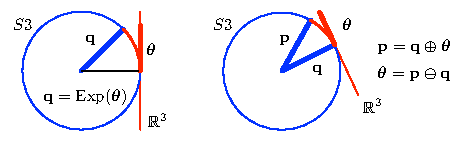
\includegraphics{figures/manifold}
\caption{The $S^3$ manifold is a unit sphere in $\bbR^4$, here represented by a unit circle (blue),  where all unit quaternions live. The tangent space to the manifold is the hyperplane $\bbR^3$, here represented by a line (red). The $\Exp()$ and $\Log()$ operators map elements of $\bbR^3$ to/from elements of $S^3$. The $\oplus$ and $\ominus$ operators relate elements of the manifold with elements in the tangent space. (Likewise, these figures illustrate the $SO(3)$ manifold.)}
\label{fig:manifold}
\end{figure}




The `plus' operator, $\oplus:S^3\times\bbR^3\to S^3$, composes a reference element $\sR\in S^3$ with a (often small) rotation specified by a vector of $\bth\in\bbR^3$ that is tangent to the $S^3$ manifold at $\sR$, yielding an element $\sS\in S^3$ (see \figRef{fig:manifold}, right). 
The `minus' operator, $\ominus:S^3\times S^3\to\bbR^3$ is the inverse of the above.
These operators are defined for both $\bfq$ and $\bfR$,
%
\begin{align}
\bfq =\, \bfp\oplus\bth  &\te \bfp\ot\Exp(\bth) \label{equ:plus_q} \\
\bfS = \bfR\oplus \bth &\te \bfR\Exp(\bth) \label{equ:plus_R} \\
\bth =\, \bfq\ominus\bfp &\te \Log(\bfp^*\ot\bfq) \label{equ:minus_q}\\
\bth = \bfS\ominus\bfR &\te \Log(\bfR\tr\,\bfS)  \label{equ:minus_R}
~.
\end{align}


%%%%%%%%%%%%%%%%%%%%%%%%%%%%%%%%%%%%%%%%%%%%%%%%%%%%%%%%%%%%%
\subsection{The four possible derivative definitions}

For functions $f:\bbR^m\to\bbR^n$, the derivative is defined classically using the standard operators $\{+,-\}$,
%
\begin{align}\label{equ:derivative_vector}
\dpar{f(\bfx)}{\bfx} &\te \lim_{\delta\bfx\to0}\frac{f(\bfx+\delta\bfx)-f(\bfx)}{\delta\bfx} &&\in \bbR^{n\times m} 
~;
\end{align}
%
for functions $g:S^3\to S^3$, we use the operators $\{\oplus,\ominus\}$,
%
\begin{align}\label{equ:derivative_SO3}
\dpar{g(\sR)}{\bth} 
&\te \lim_{\delta\bth\to0}\frac{g(\sR\oplus\delta\bth)\ominus g(\sR)}{\delta\bth}  && \in \bbR^{3\times 3}
~;
\end{align}
%
for functions $h:\bbR^m \to S^3$, we use $\{+,\ominus\}$,
%
\begin{align}\label{equ:dif_RtoSO3}
\dpar{h(\bfx)}{\bfx} &\te \lim_{\delta\bfx\to0} \frac{ h(\bfx+\delta\bfx)\ominus h(\bfx)}{\delta\bfx} && \in \bbR^{3\times m} 
~;
\end{align}
%
and for functions $k:S^3\to\bbR^n$, we use $\{\oplus,-\}$,
%
\begin{align}\label{equ:jacobian_SO3_Rn}
\dpar{k(\sR)}{\bth} &\te \lim_{\delta\bth\to0} \frac{k(\sR\oplus\delta\bth) - k(\sR)}{\delta\bth} && \in \bbR^{n\times 3} 
~.
\end{align}
%
It might be worth noticing that all these Jacobians are independent of the representation chosen ($S^3$ or $SO(3)$).


%%%%%%%%%%%%%%%%%%%%%%%%%%%%%%%%%%%%%%%%%%%%%%%%%%%%%%%%%%%%%
\subsection{Right Jacobian of $S^3$ and $SO(3)$}

We define the right Jacobian as, 
%
\begin{align}\label{equ:Jr}
\bfJ_r(\bth) &\te \dpar{\Exp(\bth)}{\bth} 
\in\bbR^{3\tcross^3}
~,
\end{align}
%
and implement it using \eqRef{equ:dif_RtoSO3}.
It admits the closed form  \cite[pag.~40]{CHIRIKJIAN-12}, 
%
\begin{align}
\bfJ_r(\bth) &= \bfI - \frac{1-\cos\nth}{\nth^2}\hatx{\bth} + \frac{\nth-\sin\nth}{\nth^3}\hatx{\bth}^2 
~.
\end{align}



%%%%%%%%%%%%%%%%%%%%%%%%%%%%%%%%%%%%%%%%%%%%%%%%%%%%%%%%%%%%%
\subsection{Examples}

\subsubsection{Function $\bbR^3\to S^3$} 
\label{sec:jac_R3toSO3}

The function $f(\bw) = \Exp(\bw\dt)$ produces elements of $S^3$ from vectors $\bw\in\bbR^3$. 
Its Jacobian \wrt $\bw$ follows from \eqRef{equ:dif_RtoSO3}, also obtained from \eqRef{equ:Jr} and the chain rule,
%
\begin{align*}
\dpar{\Exp(\bw\dt)}{\bw}
= \dpar{\Exp(\bw\dt)}{(\bw\dt)}\dpar{(\bw\dt)}{\bw} 
= \bfJ_r(\bw\dt)\dt
~.
\end{align*}
%


\subsubsection{Function $S^3\times\bbR^3\to\bbR^3$} 
\label{sec:jac_SO3xR3toR3}

The rotation $f(\sR,\bfv) = \bfq\od\bfv = \bfR\,\bfv$ produces vectors of $\bbR^3$ from elements $\sR\in S^3$ and vectors $\bfv\in\bbR^3$. The first Jacobian is defined by \eqRef{equ:jacobian_SO3_Rn} and developed as
%
\begin{align*}
\dpar{\bfq\od\bfv}{\bth} = \dpar{\bfR\bfv}{\bth} 
&\te \lim_{\delta\bth\to0}\frac{(\bfR\oplus\delta\bth)\bfv-\bfR\bfv}{\delta\bth} \\
= \lim_{\delta\bth\to0}\frac{\bfR\Exp(\delta\bth)\bfv-\bfR\bfv}{\delta\bth} 
&= \lim_{\delta\bth\to0}\frac{-\bfR\hatx{\bfv}\delta\bth}{\delta\bth} 
= -\bfR\hatx{\bfv} 
\end{align*}
%
where we used the properties $\Exp(\dth) \approx \bfI + \hatx{\dth}$ and  $\hatx{\bfa}\bfb = -\hatx{\bfb}\bfa$. 
The second Jacobian is defined by \eqRef{equ:derivative_vector} and yields,
%
\begin{align*}
\dpar{\bfq\od\bfv}{\bfv} = \dpar{\bfR\bfv}{\bfv} 
&\te \lim_{\partial\bfv\to0}\frac{\bfR\tdot(\bfv+\partial\bfv)-\bfR\bfv}{\partial\bfv} 
= \bfR
~.
\end{align*}

%%%%%%%%%%%%%%%%%%%%%%%%%%%%%%%%%
\subsubsection{Function $S^3\times S^3\to S^3$}
\label{sec:jac_SO3xSO3toSO3}

The function $f(\sQ,\sR) = \bfq\ot\bfr = \bfQ\,\bfR$ produces rotation composition. Its Jacobians are computed from \eqRef{equ:derivative_SO3}, using the property $\Exp(\bfR\bth)=\bfR\Exp(\bth)\bfR\tr$,
%
\begin{align*}
\dpar{\bfq(\bftheta)\ot\bfr}{\bftheta} 
=
\dpar{\bfQ(\bftheta)\,\bfR}{\bftheta} 
&= \lim_{\delta\bftheta\to0}\frac{\Log\big((\bfQ\bfR)\tr(\bfQ\Exp(\delta\bftheta)\bfR)\big)}{\delta\bftheta} \\
&= \lim_{\delta\bftheta\to0}\frac{\Log\big(\bfR\tr\Exp(\delta\bftheta)\bfR\big)}{\delta\bftheta} 
%&= \lim_{\delta\bftheta\to0}\frac{\Log\big(\Exp(\bfR\tr\delta\bftheta)\big)}{\delta\bftheta} 
= \bfR\tr
~,
\\
\dpar{\bfq\ot\bfr(\bfphi)}{\bfphi} 
=
\dpar{\bfQ\,\bfR(\bfphi)}{\bfphi} 
&= \lim_{\delta\bfphi\to0}\frac{\Log\big((\bfQ\bfR)\tr(\bfQ\bfR\Exp(\delta\bfphi))\big)}{\delta\bfphi} \\
&= \lim_{\delta\bfphi\to0}\frac{\Log\big(\Exp(\delta\bfphi)\big)}{\delta\bfphi} 
= \bfI
~.
\end{align*}




